\documentclass[conference]{IEEEtran}
\IEEEoverridecommandlockouts
% The preceding line is only needed to identify funding in the first footnote. If that is unneeded, please comment it out.
\usepackage{cite}
\usepackage{url}
\usepackage{amsmath,amssymb,amsfonts}
\usepackage{algorithmic}
\usepackage{graphicx}
\usepackage{textcomp}
\usepackage{xcolor}
\def\BibTeX{{\rm B\kern-.05em{\sc i\kern-.025em b}\kern-.08em
    T\kern-.1667em\lower.7ex\hbox{E}\kern-.125emX}}
\begin{document}

\title{Network Data Collection for Artificial Intelligence}

\author{\IEEEauthorblockN{Sebastian Lipp}
\IEEEauthorblockA{\textit{IT Security} \\
\textit{FH Technikum Wien}\\
Vienna, Austria \\
cs19m032@technikum-wien.at}
\and
\IEEEauthorblockN{Damir Marijanovic}
\IEEEauthorblockA{\textit{IT Security} \\
\textit{FH Technikum Wien}\\
Vienna, Austria \\
cs19m031@technikum-wien.at}
\and
\IEEEauthorblockN{Boris Stampf}
\IEEEauthorblockA{\textit{IT Security} \\
\textit{FH Technikum Wien}\\
Vienna, Austria \\
cs19m006@technikum-wien.at}
}

\maketitle

\begin{abstract}
Collecting real network data for further processing is an important topic for the training of neural networks which filter suspicious from ordinary traffic. This paper focuses mainly on research in the areas of network simulation, network recording and data extraction which should serve as input for the following papers.
\end{abstract}

\begin{IEEEkeywords}
artificial intelligence, neural networks, computer networks, network security, data collection
\end{IEEEkeywords}

\section{Introduction}
Neural networks which filter suspicious network traffic need a training data set of high quality. This data set could be produced from real network traffic but this can be difficult to implement. Another option considers network simulators which can be easily configured depending on the selected scenarios.

This paper is split in three chapters. The first chapter compares available network simulators and their software interfaces and explores possibilities for their automated setup based on the scenario and parameters. The second chapter focuses on tools to record the network traffic. In the third chapter methods of feature extraction and label definition are covered. This information serves as foundation for the further implementation of a system for automated data collection for artificial intelligence.

At this point all our considerations are based on theoretical research  without practical implementation which will come to life in further work. Therefore this paper sets a direction and foundation for the next steps and shows possible solutions on a high level.

\section{Simulation}

Before network simulators can be compared the requirements have to be defined. Because the produced network traffic should be close to real traffic it would be advisable to choose a network simulator which works with the simulation of real network equipment and can also integrate real hardware or virtual machines into the simulation which is necessary to redirect the network traffic to the recorder and data extractor. This is important to consider since other simulators like NS3 provide discrete-event network simulation which is a needless complexity overhead for this kind of application. It would be desirable if they are affordable and provide an easy-to-use interface to create and control specific network topologies through a programming language like Python to automate their creation. Moreover they should be resource-efficient and easy to deploy. The provisioning of the simulation hosts has to be simple and also scalable to be prepared for simulating denial-of-service attacks.

The next sections cover possible network simulators, system environments and the provisioning of the infrastructure.

\subsection{Comparing common network simulators}
There are many solutions available on the market to simulate networks. Popular network simulators which possibly fulfill the requirements above are for example VIRL, GNS3 or EVE-NG. This section focuses on the comparison of these simulators and the selection of the best solution for our use case.  \cite{b1}

\begin{figure}[htbp]
\centerline{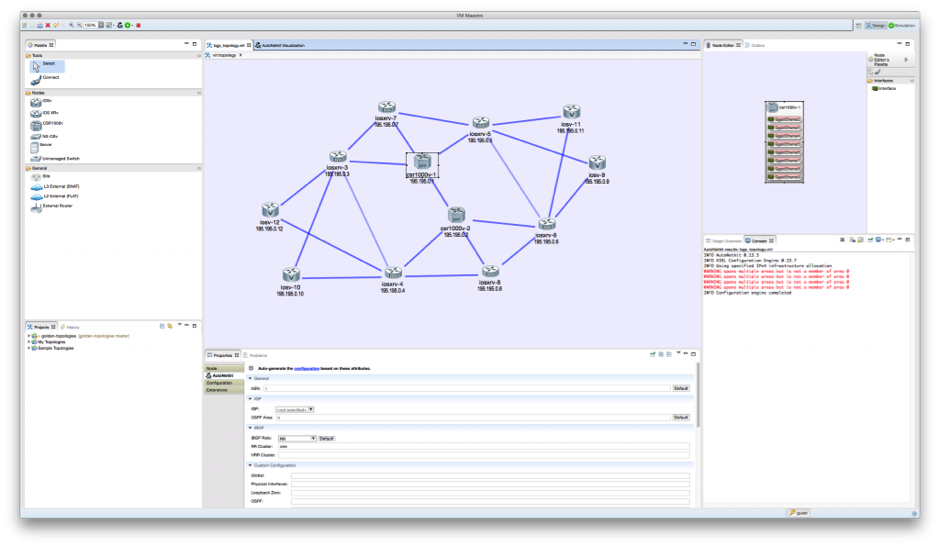
\includegraphics[scale=0.55]{virl.png}}
\caption{Sample network topology in VIRL \cite{b2}}
\label{virl}
\end{figure}

VIRL (Cisco Virtual Internet Routing Lab) is a network modeling and simulation environment provided by Cisco which offers the ability to use simulation models of real Cisco platforms, integrate virtual machines and connect real networks. Furthermore it provides a RESTful API to configure networks without a graphical interface, sufficient documentation and scalability as well as easy deployment through prepared images. It is not for free and only supports VMware or bare-metal installs. Simulation models of other vendors are not supported. Tests in virtual machines unveiled a good responsiveness but a long topology loading time with high CPU load. Fig.~\ref{virl} shows a sample network topology created via the graphical user interface of VIRL.  \cite{b1} \cite{b3}

\newpage

\begin{figure}[htbp]
\centerline{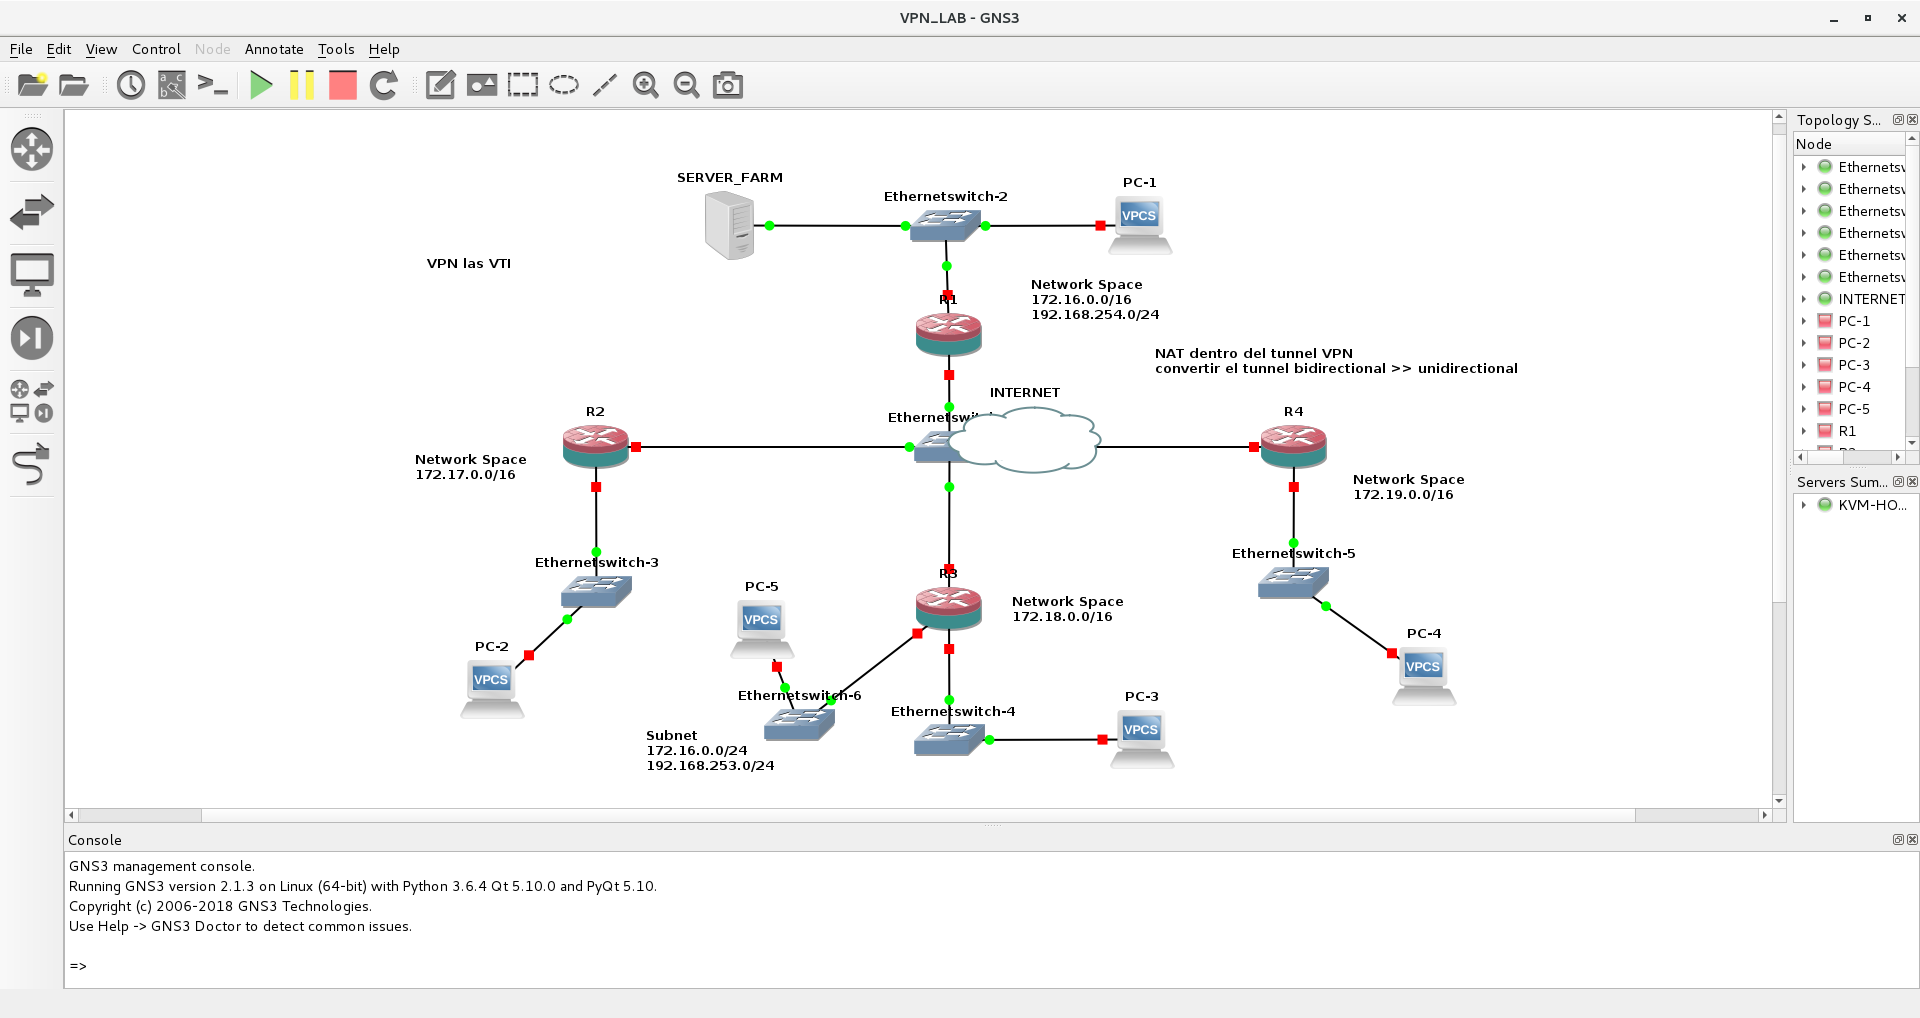
\includegraphics[scale=0.13]{gns3.png}}
\caption{Sample network topology in GNS3 \cite{b4}}
\label{gns3}
\end{figure}

GNS3 (Graphical Network Simulator 3) is a very popular free open source software to emulate and test networks. It offers the integration of virtual machines and real networks and supports models of various vendors but does not offer pre-installed device images due to license issues. It also provides a RESTful API to set up network topologies, a big community and scalability. The software can be easily installed through packages on all operating systems and supports all hypervisors as well Docker containers. Performance tests showed a long topology loading time with high CPU load but a good response through the user interface. Fig.~\ref{gns3} shows a sample network topology created with GNS3.  \cite{b1} \cite{b5}

\begin{figure}[htbp]
\centerline{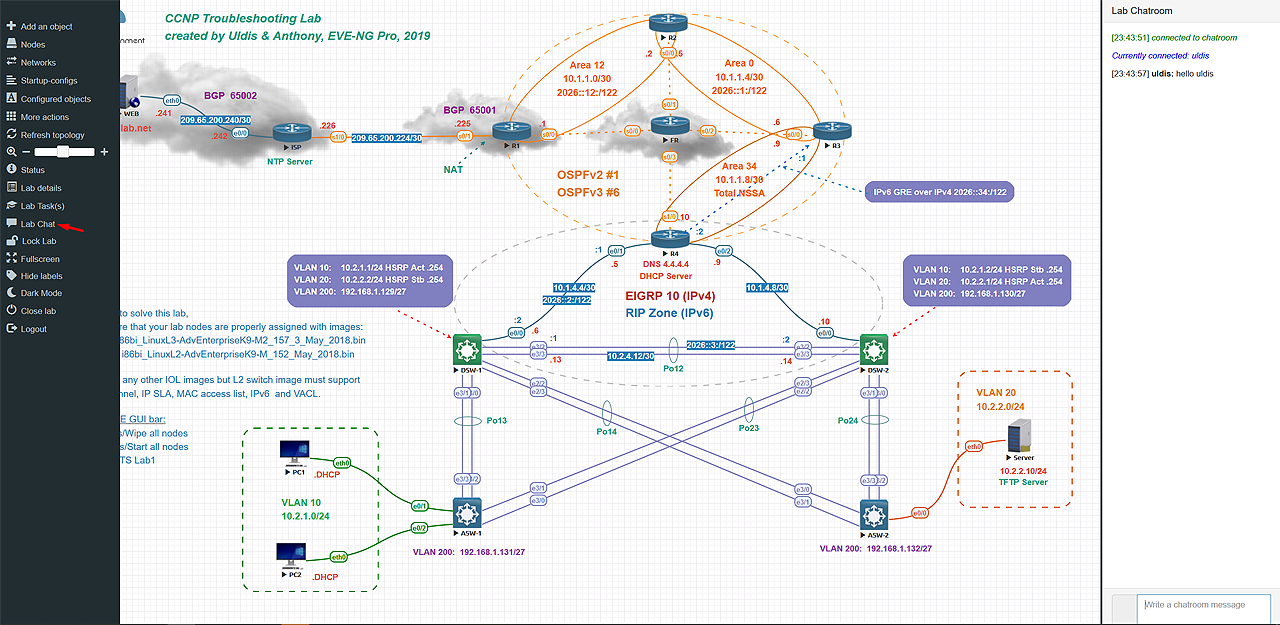
\includegraphics[scale=0.19]{eve-ng.png}}
\caption{Sample network topology in EVE-NG \cite{b6}}
\label{eve-ng}
\end{figure}

EVE-NG (Emulated Virtual Environment - Next Gen) is a network emulator which comes in a free and a professional edition and offers the interaction with real networks. It supports multiple vendors but does not provide device images. Advanced features like Docker, configuration management or Wireshark integration only come with the purchase version. Moreover a RESTful API and images for the installation in virtual machines are available as well as a reasonable documentation. The software is scalable and performs well in virtual machines with a short topology loading time and provides an intuitive interface as shown in Fig.~\ref{eve-ng}.  \cite{b1} \cite{b7}

All solutions are very similar in their functionalities but distinguish in their vendor support, performance, documentation and price. VIRL only supports Cisco devices but comes with device images like GNS3 and EVE-NG support various vendors but do not ship images. But many proprietary and open source images are available on the internet for free. VIRL and EVE-NG are propriatary like GNS3 is free and open source. EVE-NG performs better in virtual machines than VIRL and GNS3.

Regarding these factors GNS3 fullfills our requirements the most because it is free, supports all vendors and comes with a big community and documentation. Our second option could be EVE-NG in the professional edition which also supports all vendors.

\subsection{Selecting the deployment environment}

Next steps include the integration of the selected network simulator in a scalable environment which can be set up easily. 

\begin{figure}[htbp]
\centerline{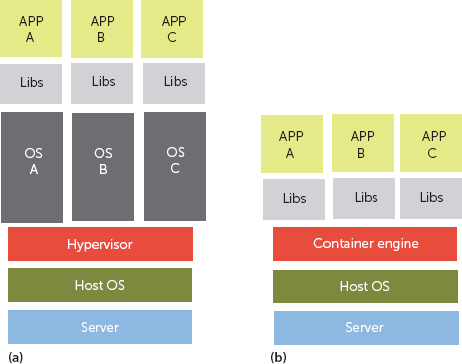
\includegraphics[scale=0.5]{docker_vm.png}}
\caption{Virtual machines vs. Containers \cite{b8}}
\label{docker-vm}
\end{figure}

Hypervisors like VirtualBox or VMware provide the possibility to set up full virtual computers on a physical host (see Fig.~\ref{docker-vm}a) while Docker containers are encapsuled sandboxes on an existing operating system (see Fig.~\ref{docker-vm}b). It is clear that containers are more resource efficent but in virtual machines the systems are better isolated. In our case we could use both solutions because the network simulators are also capable to run in Docker containers. If we focus on resource efficency and scalability also Kubernetes comes in our minds which is an orchestrator for deploying Docker containers on multiple nodes but it is a more complex configuration overhead and needs certain amount of hardware to unfold its potential also for simple scenarios. Because we want an affordable solution which can be used in most of the cases also on our computers with some exceptions, we could use a tool which can create virtual machines as well as Docker containers to be ready for the future. Regarding the corner cases servers or a Kubernetes cluster could be rented temporarily on cloud platforms like AWS to support high-load scenarios e.g. big denial-of-service attacks. \cite{b8}

A popular solution to bootstrap development environments in virtual machines is called Vagrant which provides lightweight base images and an interface to automate the configuration of the virtual machines. Moreover it can be connected to provisioning tools to further configure host systems. Vagrant supports VirtualBox or VMware but also Docker and can be extended to support cloud services like AWS or even to install a whole Kubernetes cluster. It gives us the power to start with simple configurations and scale them up to more sophisticated ones using containerization and complex orchestrators. \cite{b9} \cite{b10}

This means we would be ready to create system environments on our host or in the cloud and install base systems on them. The next section focuses on the automated setup of the network simulator, recorder and data extractor within virtual machines or Docker containers as well as the configuration of network topologies based on the selected scenarios and parameters to produce, record and extract network traffic for further processing in neural networks to improve their strike rate.

\subsection{Provisioning of the infrastructure}

Vagrant supports multiple provisioners like Ansible, Terraform or simple bash scripts to configure the host systems and can also be set up through them. For the beginning we could use Ansible through Vagrant to configure the host system. Vagrant can set up multiple virtual machines or Docker containers on one host. If we would need to set up machines on multiple hosts we could come back to tools like Terraform for example. \cite{b9} \cite{b10} \cite{b11}

If all the possible network scenarios are defined these network topologies have to be deployed through our deployment system. This means we could define the basic host setup and the network configurations for all the scenarios in Ansible templates which could be later adjusted via command line parameters. The topology can then be deployed by executing a shell command. This includes the deployment of the network recorder and the data extractor. In other words one or multiple scenarios can be started and connected to one recorder and data extractor to combine simultaneous attacks and everything will be deployed through a shell command with static configuration in templates and dynamic configuration with command line options. It will be also possible to integrate real hardware into the simulation. \cite{b9}

\begin{figure}[htbp]
\centerline{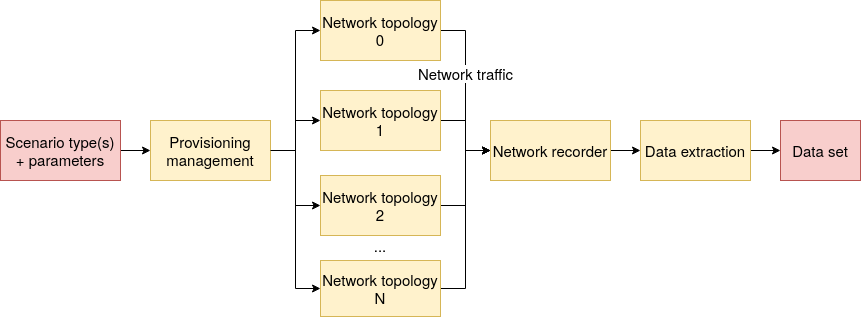
\includegraphics[scale=0.28]{design_flow.png}}
\caption{Data collection workflow}
\label{design-flow}
\end{figure}

Fig.~\ref{design-flow} shows a possible simulation workflow. The input parameters are the type of scenario(s) and the respective settings which deploys hosts including the base systems and the simulators applying the network topologies. Moreover the network recorder and data extractor could be deployed to gather the network traffic and extract the features to create data sets which could be collected in a central database.

A real test case would then consist of multiple scenarios of attacks and usual network traffic recorded, extracted and collected in a central place. The next chapter focuses on recording the generated data.

\section{Recording}

Before the network traffic can be analysed, it has to be recorded first. Therefore, this chapter will give an overview of the available third-party software which can be used to record all the incoming network traffic. The functional requirements for a tool are chiefly the pace of handling the network traffic. All of these tools are client-based tools. This means that either the network target for the traffic has to be a client or the e.g. switch has to clone a port with all the incoming and outgoing traffic and direct all the data to a client running one or more of these tools. In some cases, analysing of network traffic can take much longer than the data is sent or received by the network which means, that all the data need to be buffered or stored. In this case a packet-to-disk recorder is needed. This device can capture large amount of network traffic with a data rate of up to 40 Gbit/s and write it into files. 

\subsection{pcap Library}

Every tools needs APIs\footnote{Application Programming Interface} to capture all the traffic sent through the network interface. Therefore, libraries were made for both Unix-like and Windows based operating systems. While \textit{libpcap} is used for Unix-like operating systems, a Windows system needs the library called \textit{WinPcap}. In 2013 the last release (4.1.3) of \textit{WinPcap} was published. Since then \textit{Npcap} acts as a substitute\cite{winpcaporg}. With a pcap library, software has the ability to tap all the network traffic from the selected interface. Based on the possibility to include the library in \textbf{C} and \textbf{C++}, \textit{pcap} can be used very easily in software. With the release of \textit{libpcap} 1.0.0, the zero-copy mechanism was implemented which allows the software to read the network traffic directly without copying the data from kernel space to user space.

\subsection{Network Recording Tools}

In this section we will itemise five well known and useful network recording tools. Some of the tools are console based tools, others have a GUI, or both.

\subsection*{tcpdump}

Especially in the world of Unix based operating systems, \textit{tcpdump} is one of the best known tools for monitoring and sniffing network traffic. \textit{tcpdump} is an exclusively command line based tool. This property makes \textit{tcpdump} a tool for advanced command line users only. But once you get familiar with the commands and options of \textit{tcpdump}, it will get a  a very efficient and powerful tool for many applications. \textit{tcpdump} uses the \textit{libpcap} network library of Unix based operating systems for capturing network traffic.

\begin{figure}[htbp]
\centerline{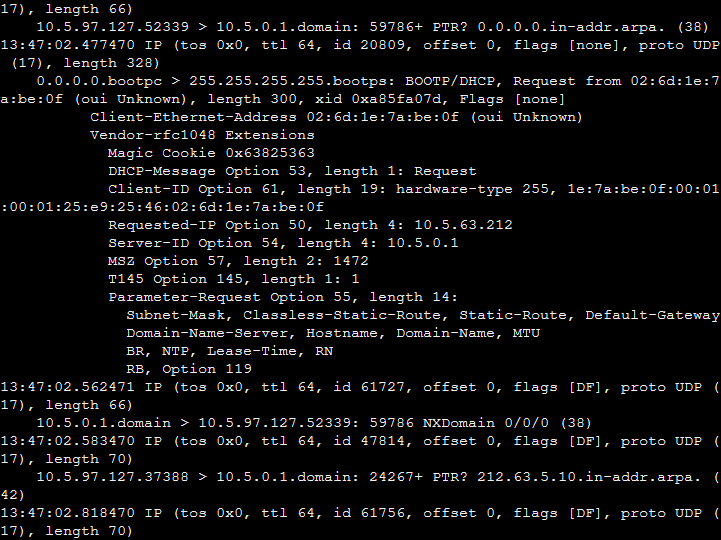
\includegraphics[scale=0.4]{tcpdump.png}}
\caption{tcpdump Network Capture}
\label{tcpdump}
\end{figure}

With the wide set of options, \textit{tcpdump} is a pretty agile tool for dumping and analysing network traffic. A few of the options are listed below \cite{tcpdumporg}. 

\begin{itemize}
\item \textbf{-i eth0} the traffic from the interface \textit{eth0} is captured
\item \textbf{-w example.dump} all the output is written into a declared file
\item \textbf{-e} the ethernet header will recorded too
\item \textbf{-r example.dump} parsing the file \textit{example.dump} into tcpdump
\end{itemize}

If \textit{tcpdump} is compiled with cryptography, it is able to decrypt IPsec ESP packets in real time \cite{goyal2017}.
For the Windows enthusiasts a Windows derivative of \textit{tcpdump} is available. It is called \textit{WinDump}. \textit{WinDump} uses the \textit{WinPcap} library, which provides the same API for Windows operating systems as \textit{libpcap} for Unix-like systems. This means, network traffic captured, e.g. on a Ubuntu system can be analysed on a Windows 10 Client afterwards.

\subsection*{Wireshark}

\textit{Wireshark} is for good reason the best known cross-platform networking tool available. In 2006 \textit{Wireshark} was started as a fork of the software called \textit{Ethereal} by the Wireshark-Community due to trademark issues \cite{asrodiapatel2012}.  The performance of this tool is powerful and the set of functions is neatly arranged. By using the GTK toolkit, \textit{Wireshark} has implemented a GUI \footnote{Graphical User Interface}\cite{suribatra2012}. The GUI is separated typically into three segments: the traffic overview, and the details and raw data of the selected packet.

\begin{figure}[htbp]
\centerline{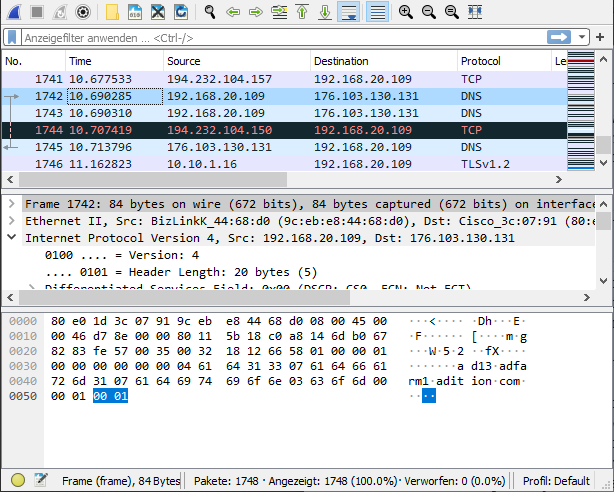
\includegraphics[scale=0.48]{wireshark.png}}
\caption{Wireshark Network Capture}
\label{wireshark}
\end{figure}

A good asset of \textit{Wireshark} is its available set of filters for capturing and displaying network data. With the help of plugins, \textit{Wireshark} can even handle with new or dedicated protocols. Another big asset of \textit{Wireshark} is its capability of capturing raw USB traffic from an USB port. By highlighting the traffic with different colours as shown in Fig.~\ref{wireshark} it's easier to scan for required traffic.

\subsection*{netsniff-ng}

\textit{netsniff-ng} is a another Unix based tool for network analysis. \textit{netsniff-ng} was the first tool which had the ability to analyse the whole traffic with a zero-copy procedure, which means that \textit{netsniff-ng} uses the same data as the kernel does. Based on this functional principle, \textit{netsniff-ng} is one of the best performing tools for network sniffing. \textit{netsniff-ng} is like \textit{tcpdump} exclusively an console based software. The set of options contains 38 capabilities on the latest version 0.6.4 of \textit{netsniff-ng}.

\subsection*{Capsa}

The fourth tool is called \textit{Capsa} from \textit{Colasoft} founded 2001 in United States. \textit{Capsa} is suitable for real-time network data capturing both LAN and Wireless Interfaces. A big advantage of \textit{Capsa} is the ability to evaluate the network traffic into graphical output like diagrams. This feature can help identifying the source of undesirable network traffic quickly by a human. The free version of \textit{Capsa} is heavily restricted regarding available functions. 

\begin{figure}[htbp]
\centerline{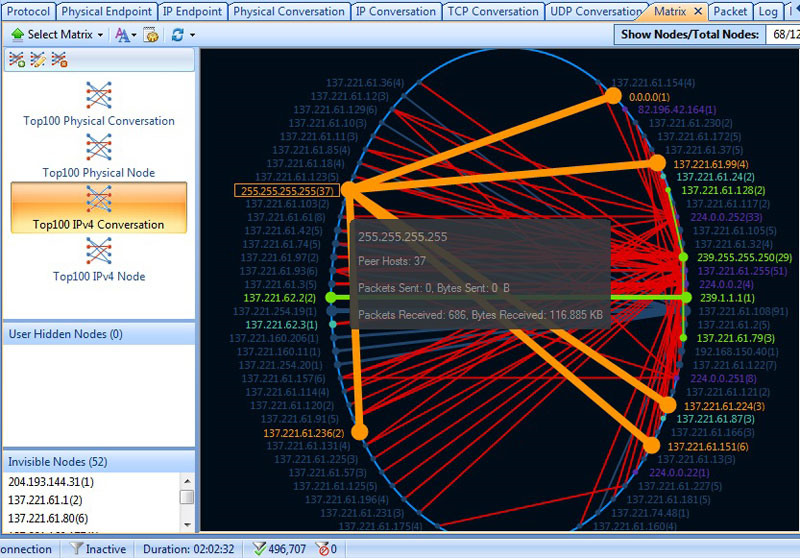
\includegraphics[scale=0.30]{capsa.png}}
\caption{Graphical Evaluation of Network Traffic with Capsa \cite{firewallcx}}
\label{capsa}
\end{figure}

\subsection*{EtherApe}

Yet another tool for network monitoring is called \textit{EtherApe}. \textit{EtherApe} is an Unix based software with a meaningful graphic interface and graphical data output of network traffic. With the help of graphical illustration anomalies like a DDoS attack can be detected easily as shown in Fig.~\ref{etherape}. Every host is shown as a node in circle, every connection is shown as link between two nodes and every protocol has an own colour for the link. With higher network traffic between two hosts the link between nodes is shown larger.

\begin{figure}[htbp]
\centerline{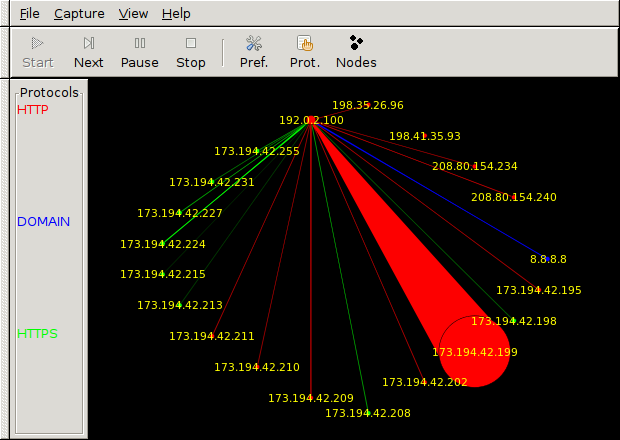
\includegraphics[scale=0.37]{etherape.png}}
\caption{Graphic Representation of Network Traffic \cite{etherapewiki}}
\label{etherape}
\end{figure}

\section{Data Extraction}

Datasets for intrusion detection are often based on network packet data captured by sniffers, which can be stored in pcap files (as done in the UNSW-NB15 \cite{Nb2015} and CSE-CIC-IDS2018 \cite{Ids2018} datasets). Before a machine learning algorithm can be employed, features have to be extracted from the captured data. A wide range of different features is described in literature. For the sake of clarity, these features are divided into groups which are described in the following subsections.

There also exists a large number of techniques for dimensionality reduction. The 40 features of the NSL-KDD data set could be reduced to 30 or 16 features, with no or low degradation in detection power. The benefits of a reduced feature set are faster processing, less memory consumption, and in some cases even higher detection precision, because some classifiers have problems with irrelevant or correlated features. This could be achieved by combining the following methods \cite{vasquez2015}:
\begin{itemize}
	\item Weight by maximum relevance
	\item Minimum redundancy maximum relevance
	\item Significance analysis for microarrays
	\item Least absolute selection and shrinkage operator
	\item Stability selection
	\item Stepwise regression
\end{itemize}

Other methods which can be used for that purpose are based on association rule mining (ARM) \cite{moustafa2015}, sequential forward selection (SFS) \cite{dehghani2010} \cite{xu2015}, or the T-test \cite{sopuru2019}, 

When selecting the features, their limitations should be considered as well. Some features can easily be spoofed by attackers, while others are unable to detect encrypted malware traffic or cause performance problems. The development of new evasion techniques (e.g., disguising malicious traffic in widely used protocols such as HTTP) make the detection even harder \cite{celik2015}.

Another aspect which has been examined is the stability of features in terms of time (year 2000/2001 vs. 2008) and location (Internet core vs. Internet edge). In this regard, the packet size can be considered as stable feature \cite{este2009}. The suitability of features also depends on the type of network which is analyzed. For example, some industrial control system networks are relatively static regarding IP address allocation, the number of open connections and the ports, protocols and settings they use. Therefore, features based on these attributes may provide good results in that particular environment \cite{mantere2013}.

\subsection{Flow statistical features}

A common approach is to group packets into flows, and then calculate statistical features based on these flows. Generally, a flow is a group of packets with the same source and destination IP addresses and ports, and the same protocol. However, a flow can also be terminated by a TCP FIN packet or a timeout \cite{Ids2018}. Statistical features of network flows include the following:
\begin{itemize}
	\item Flow duration \cite{Nb2015} \cite{Ids2018}
	\item Time between two flows or packets \cite{Ids2018}
	\item Time between SYN and SYN/ACK, and between SYN/ACK and ACK packets during TCP connection setup \cite{Nb2015}
	\item Active time before a flow becomes idle and vice versa \cite{Ids2018}
	\item Jitter \cite{Nb2015}
	\item Number of packets in total, with at least 1 byte of payload, or with certain protocol flags \cite{Ids2018} \cite{waizumi2007} \cite{celik2015}
	\item Number of fragmented packets \cite{waizumi2007}
	\item Number of retransmitted or dropped packets \cite{Nb2015}
	\item Size of packets, payload, headers or segments \cite{Ids2018} \cite{celik2015}
	\item Number of bytes/packets transferred per second, in bulk, or in the initial TCP window \cite{Ids2018} \cite{celik2015}
	\item Number of RTT samples \cite{celik2015}
	\item Time to live value \cite{Nb2015}
	\item TCP window advertisement value \cite{Nb2015}
	\item TCP base sequence number \cite{Nb2015}
	\item Ratio between download and upload \cite{Ids2018}
	\item Ratio between maximum and minimum packet size \cite{celik2015}
	\item Number of flows with the current flow's IP address or port number \cite{waizumi2007} \cite{Nb2015}
\end{itemize}
Most of these features can be derived by statistical calculations such as total, minimum, maximum, mean, median, standard deviation, variance, skewness and kurtosis \cite{Ids2018} \cite{celik2015, xu2015}. Also, the features can be extracted from bidirectional flows, or separately for forward and backward directions \cite{Ids2018}.

The open-source Java software CICFlowMeter can be used to extract features of network flows (which end either by TCP FIN packet, or a configurable timeout) from pcap files. It allows to select from a list of available features, but can also be extended to support new features \cite{cicflowmeter}, and has therefore been used in various applications \cite{Ids2018} \cite{lashkari2017} \cite{sopuru2019}.

\begin{figure}[htpb]
\centerline{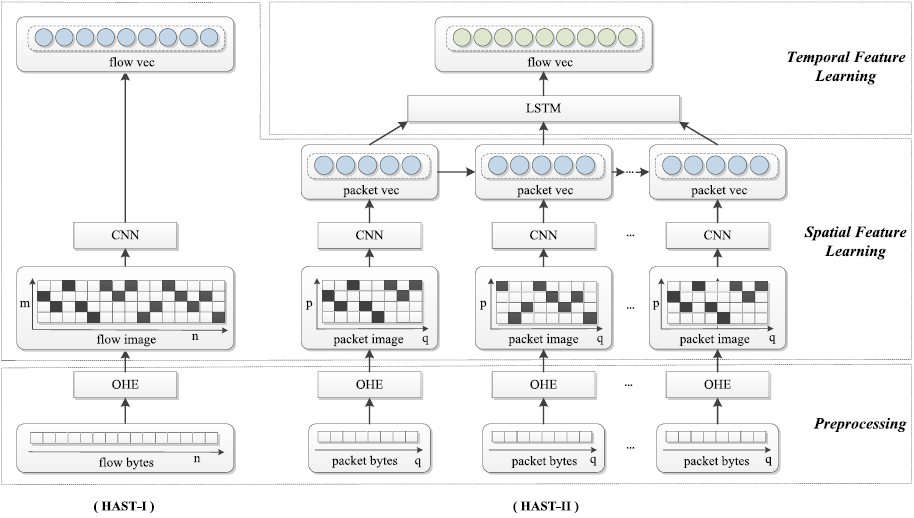
\includegraphics[scale=0.35]{hast-ids.png}}
\caption{Feature learning process of HAST-IDS \cite{wang2018}}
\label{hast-ids}
\end{figure}

The hierarchical spatial-temporal feature-based intrusion detection system (HAST-IDS), which is shown in fig.~\ref{hast-ids}, also extracts flow-based features. However, it first transforms the bytes of network flows (HAST-I) or packets (HAST-II) into images using one-hot encoding (OHE), and then uses deep convolutional neural networks (CNNs) and long short-term memory (LSTM) networks to learn features based on these images \cite{wang2018}.

\subsection{Timeslot features}

Timeslot features are extracted by counting the number of certain events in fixed time intervals. For the detection of DoS and probing traffic, the following timeslot features are proposed \cite{waizumi2007}:
\begin{itemize}
	\item Number of TCP, UDP and ICMP packets
	\item Number of bytes sent and received through all TCP connections
	\item Number of TCP ports
	\item Number of occurences of TCP flags
	\item Number of DNS packets
	\item Number of fragmented packets
	\item Number of values of the four fields of IP addresses
\end{itemize}

\subsection{Behavioral features}

A different approach is to define features which measure specific behavioral differences between benign and malicious software.

One system following that approach is called "traffic aggregation for malware detection". It defines three characteristics which can be combined to distinguish between benign and malware traffic \cite{yen2011}:
\begin{itemize}
	\item Common destinations (assuming that compromised systems contact different hosts than uncompromised systems)
	\item Similar payload (assuming that command-and-control traffic uses common protocol syntax)
	\item Common software platforms (assuming that malware usually relies upon a specific operating system and also specific applications, such as web browsers)
\end{itemize}

The UNSW-NB15 datasets contains mostly flow statistical features, but also a few features based on behavior \cite{Nb2015}:
\begin{itemize}
	\item A binary value denoting if the source and destination IP addresses and port numbers are equal
	\item Service (HTTP, FTP, SMTP, SSH, DNS, or IRC)
	\item Pipelined depth into the connection of HTTP request/response transaction
	\item Actual uncompressed content size of the data transferred from the server's HTTP service
	\item Number of flows containing HTTP GET and POST methods
	\item A binary value denoting if a FTP session is accessed by user and password
	\item Number of flows containing FTP commands
\end{itemize}

Reference \cite{li2013} lists the following features which can be used for detecting communication with known and unknown botnets:
\begin{itemize}
	\item Accessing the main and backup DNS server at the same time (benign software would only access the backup DNS server if the main DNS server is not available)
	\item Resolving a specific domain name periodically
	\item Accessing a fast-flux service network (FFSN)
	\item Downloading malicious binary code (which can be checked using antivirus software)
	\item Scanning for open ports
	\item Periodically creating null TCP connections (zero TCP window or IRC PING/PONG connections which are used for contacting the command and control server)
\end{itemize}

Similarily, the character code distribution of payloads can be used to detect buffer overflow traffic (where some character codes have exceptionally high frequency) \cite{waizumi2007}.

\subsection{Host-based features}

The previous sections examined different features which can be extracted from network traffic, but there are also host-based data which can be used for intrusion detection. These include operating system event logs \cite{Ids2018} and other log files (e.g., firewall, mail and FTP logs) \cite{abad2003}.

A different approach is the use of features derived from raw system call traces. The advantage of system call traces over log files is that they contain only raw information about the interaction between programs and the operating system kernel, whereas log files contain data interpreted by various programs, and potentially include large amounts of irrelevant data. There are multiple methods of analysing system calls. Some only look at the pattern of system calls, while others also look at the arguments passed to these system calls. Also, there is a distinction between syntactic features, which depend only on contiguous patterns of system calls, and semantic features, which additionally consider the meaning of system call arguments or groups of discontiguous system calls. The advantage of the semantic approach is that it is able to counter mimicry attacks, where the payload is modified by the attacker with the aim that the system calls it executes cannot be classified as being malicious \cite{creech2014}.

\subsection{Label definition}

In addition to the feature vectors, datasets to be used for supervised learning need to include labels. For the purpose of intrusion detection, each record (e.g., network flow) has to be labelled  binary as benign or malicious traffic, or nominally to distinguish between certain attack types. For example, the UNSW-NB15 dataset defines a binary label (0 for normal and 1 for attack) and a nominal label ("Normal" for benign traffic and "Fuzzers", "Analysis", "Backdoors", "DoS", "Exploits", "Generic", "Reconnaissance", "Shellcode" or "Worms" for the various attack types) \cite{Nb2015}. For some applications, there may also be a nominal label for benign traffic (e.g., browsing, chat, mail, P2P, streaming, VoIP) \cite{lashkari2017} \cite{bagui2017}.

For data generated by simulating attacks, the labels can simply be based on the schedule of simulated attacks in combination with the IP addresses, ports and protocols involved \cite{Ids2018}.

\section{Conclusion}

The quality of a dataset is generally crucial for the performance of machine learning algorithms, and generating a high quality dataset for intrusion detection systems is not a simple task. While the generation of representative benign and malicious data in itself is fundamental, the goal of this paper was to give an overview about the equally important tasks of network simulation, recording and data extraction. For each of these tasks, a variety of different approaches has been examined. Because each approach has its own strengths and limitations, they have to be evaluated individually for each application, depending on its specific requirements. Also, the further development of the Internet and the ongoing introduction of new attack techniques has to be considered, which may affect the suitability of current methods in the future and therefore cause the necessity to alter them or to develop new ones.

\begin{thebibliography}{00}
\bibitem{b1} Seifert, C. and Reißmann, S. and Rieger, S. and Pape, C. Evaluation von VIRL, GNS3 und Mininet als Virtual Network Testbeds in der Hochschullehre. 11. DFN-Forum Kommunikationstechnologien. Bonn: Gesellschaft für Informatik e.V.., pp. 103-112.
\bibitem{b2} Network Computing. (2020). Cisco VIRL: More Than A Certification Study Lab. [online] Available at: \url{https://www.networkcomputing.com/networking/cisco-virl-more-certification-study-lab} [Accessed 22 Feb. 2020].
\bibitem{b3} Virl.cisco.com. (2020). VIRL Getting Started Tutorial. [online] Available at: \url{http://virl.cisco.com/virl.apis.php} [Accessed 22 Feb. 2020].
\bibitem{b4} Gns3.com. (2020). GNS3 | The software that empowers network professionals. [online] Available at: \url{https://gns3.com/discussions/how-to-install-gns3-on-centos-7-} [Accessed 22 Feb. 2020].
\bibitem{b5} Gns3-server.readthedocs.io. (2020). Welcome to API documentation! — GNS3 2.1.22dev1-67e70c46 documentation. [online] Available at: \url{https://gns3-server.readthedocs.io/en/latest/} [Accessed 22 Feb. 2020].
\bibitem{b6} Eve-ng.net. (2020). Screenshots. [online] Available at: https://www.eve-ng.net/index.php/screenshots/ [Accessed 22 Feb. 2020].
\bibitem{b7} Eve-ng.net. (2020). EVE-NG API. [online] Available at: \url{https://www.eve-ng.net/index.php/documentation/howtos/how-to-eve-ng-api/} [Accessed 22 Feb. 2020].
\bibitem{b8} Bernstein, D. Containers and Cloud: From LXC to Docker to Kubernetes, in IEEE Cloud Computing, vol. 1, no. 3, pp. 81-84, Sept. 2014.
\bibitem{b9} Sandobalín, J. and Insfran, E. and Abrahão, S. (2020). On the Effectiveness of Tools to Support Infrastructure as Code: Model-Driven versus Code-Centric. IEEE Access. 10.1109/ACCESS.2020.2966597.
\bibitem{b10} Spanaki, P. Cloud Computing: Security Issues and Establishing Virtual Cloud Environment via Vagrant to Secure Cloud Hosts, 2018, pp. 539-553
\bibitem{b11} Ivanova, D. and Borovska, P. and Zahov, S. Development of PaaS using AWS and Terraform for medical imaging analytics, AIP Conference Proceedings, 2018
\bibitem{winpcaporg} WinPcap: News, Riverbed Technology (2010), https://www.winpcap.org/misc/copyright.htm [Accessed 26.02.2020]
\bibitem{tcpdumporg} Van Jacobson, C. Leres, S. McCanne,tcpdump.org (26.02.2020) https://www.tcpdump.org/manpages/tcpdump.1.html [Accessed 27.02.2020]
\bibitem{goyal2017} P. Goyal, A. Goyal (2017), Comparative study of two most popular packet sniffing tools-Tcpdump and Wireshark
\bibitem{asrodiapatel2012} P. Asrodia, H. Patel (2012). Analysis  of  Various  Packet  Sniffing  Tools  for Network  Monitoring  and  Analysis, ISSN  No.  (Online)  :  2277-2626
\bibitem{suribatra2012} S. Suri, V. Batra, Comparative Study of Network Monitoring Tools, International Journal ofInnovative Technology and Exploring Engineering (IJITEE)ISSN: 2278-3075,Volume-1, Issue-3, August 2012
\bibitem{firewallcx} http://www.firewall.cx/images/stories/review-capsa-enterprisev7-7.jpg [Accessed 26.02.2020]
\bibitem{etherapewiki} https://upload.wikimedia.org/wikipedia/commons/a/ae/Etherape-gui.png [Accessed 25.02.2020]
\bibitem{Nb2015} Moustafa, N. (2015). The UNSW-NB15 Dataset Description. [online] Available at: \url{https://www.unsw.adfa.edu.au/unsw-canberra-cyber/cybersecurity/ADFA-NB15-Datasets/} [Accessed 22 Feb. 2020]
\bibitem{Ids2018} Communications Security Establishment (CSE) and Canadian Institute for Cybersecurity (CIC) (2018). CSE-CIC-IDS2018 on AWS. [online] Available at: \url{https://www.unb.ca/cic/datasets/ids-2018.html} [Accessed 22 Feb. 2020].
\bibitem{vasquez2015} Vázquez Iglesias, F. and Zseby, T. (2015). Analysis of network traffic features for anomaly detection. Machine Learning, vol. 101, 2015.
\bibitem{moustafa2015} Moustafa, N. and Slay, J. (2015). The significant features of the UNSW-NB15 and the KDD99 data sets for Network Intrusion Detection Systems. 2015 4th International Workshop on Building Analysis Datasets and Gathering Experience Returns for Security (BADGERS), Kyoto, pp. 25-31, 2015.
\bibitem{dehghani2010} Dehghani, F. and Movahhedinia, N. and Khayyambashi, M. R. and Kianian, S. (2010). Real-time traffic classification based on statistical and payload content features. 2010 2nd International Workshop on Intelligent Systems and Applications, Wuhan, pp. 1-4, 2010.
\bibitem{xu2015} Xu, M. and Zhu, W. and Xu, J. and Zheng, N. (2015). Towards selecting optimal features for flow statistical based network traffic classification. APNOMS 2015 - pp. 479–482, 08 2015.
\bibitem{sopuru2019} Sopuru, J. and Sari, A. and Akkaya, M. (2019). Modeling a malware detection and categorization system based on seven network flow-based features. International Journal of Innovative Technology and Exploring Engineering (IJITEE), vol. 8(7), pp. 2982-2989, 05 2019
\bibitem{celik2015} Celik, Z. Berkay and Walls, R. J. and McDaniel, P. and Swami, A. (2015). Malware traffic detection using tamper resistant features. MILCOM 2015 - 2015 IEEE Military Communications Conference, pp. 330–335, Oct 2015.
\bibitem{este2009} Este, A. and Gringoli, F. and Salgarelli, L. (2009). On the stability of the information carried by traffic flow features at the packet level. SIGCOMM Comput. Commun. Rev., vol. 39, p. 13–18, June 2009.
\bibitem{mantere2013} Mantere, M. and Sailio, M. and Noponen, S. (2013). Network traffic features for anomaly detection in specific industrial control system network. Future Internet, vol. 5, pp. 460-473, 2013
\bibitem{waizumi2007} Waizumi, Y. and Sato, Y. and Nemoto, Y. (2007). A network-based anomaly detection system using multiple network features. Proceedings of the Third International Conference on Web Information Systems and Technologies - Internet Technology, pp. 410-413, 2007.
\bibitem{cicflowmeter} Canadian Institute for Cybersecurity (CIC) (2016). Applications | Research | Canadian Institute for Cybersecurity | UNB. [online] Available at: \url{https://www.unb.ca/cic/research/applications.html#CICFlowMeter} [Accessed 24 Feb. 2020].
\bibitem{lashkari2017} Lashkari, A. H. and Gil, G. D. and Mamun, M. S. I. and Ghorbani, A. A. (2017). Characterization of tor traffic using time based features. Proceedings of the 3rd International Conference on Information Systems Security and Privacy (ICISSP 2017), pp. 253-262, 2017.
\bibitem{wang2018} Wang, W. and Sheng, Y. and Wang, J. and and Zeng, X. and Ye, X. and Huang, Y. and Zhu, M. (2018). HAST-IDS: Learning hierarchical spatial-temporal features Using deep neural networks to improve intrusion detection. IEEE Access, vol. 6, pp. 1792-1806, 2018.
\bibitem{yen2011} Yen, T. (2011). Detecting stealthy malware using behavioral features in network traffic. PhD thesis, Carnegie Mellon University, 2011.
\bibitem{li2013} Li, W. M and Xie, S. L. and Luo, J. and Zhu, X. D. (2013). A detection method for botnet based on behavior features. Advanced Information and Computer Technology in Engineering and Manufacturing, Environmental Engineering, vol. 765 of Advanced Materials Research, pp. 1512–1517, Trans Tech Publications Ltd, 10 2013.
\bibitem{abad2003} Abad, C. and Taylor, J. and Sengul, C.  and Yurcik, W. and Zhou, Y. and Rowe, K. (2003). Log correlation for intrusion detection: a proof of concept. 19th Annual Computer Security Applications Conference, 2003. Proceedings., pp. 255–264, Dec 2003.
\bibitem{creech2014} Creech, G. and Hu, J. (2014). A semantic approach to host-based intrusion detection systems using contiguous and discontiguous system call patterns. IEEE Transactions on Computers, vol. 63, no. 4, pp. 807-819, April 2014.
\bibitem{bagui2017} Bagui, S. and Fang, X. and Kalaimannan, E. and Bagui, S. C. and Sheehan, J. (2017). Comparison of machine-learning algorithms for classification of vpn network traffic flow using time-related features. Journal of Cyber Security Technology, vol. 1, no. 2, pp. 108–126, 2017.
\end{thebibliography}


\vspace{12pt}
\color{red}
\end{document}


